\documentclass{article}
\usepackage[UTF8]{ctex}
\usepackage{amsmath}
\usepackage{graphicx}
\usepackage{cite}
\usepackage{subfigure}

\title{运用雅克比和高斯赛德尔公式的求解方程组}
\author{21级计算机科学与技术\ 陈岳阳}
\date{\today}

\begin{document}
\maketitle
\tableofcontents

\section{线性方程组的迭代法}
	线性方程组的解法可分为直接法和迭代法。迭代法的算法简单,编制程序比较容易,但是对于系数矩阵有特殊要求。

	通常,迭代法使用新值和老值的偏差刻画精度,且设置最大迭代次数防止迭代过程发散或收敛过于缓慢。
  \subsection{雅可比迭代法}
	考察一般形式的线性方程组
$$
\sum\limits^n_{j=1}a_{ij}x_j=b_i,\ k=1,2,\dots,n
$$
	分离出变量$x_i$,将其改写为:
$$
x_i=\frac{1}{a_{ii}}(b_i-\sum\limits^n_{j=1,j\neq n}a_{ij}x_j),\ i=1,2,\dots,n
$$
	由此可以建立出被称为雅可比迭代公式的迭代式:
$$
x^{(k+1)}_i=\frac{1}{a_{ii}}(b_i-\sum\limits^n_{j=1,j\neq n}a_{ij}x^{(k)}_j),\ i=1,2,\dots,n
$$
    \subsection{高斯-塞德尔迭代}
	由于我们使用雅可比迭代法得到的新值比老值更准确,因此可以将其替代老值用于下一步的迭代,这就是高斯-塞德尔迭代的思想。
$$
	x^{(k+1)}_i=\frac{1}{a_{ii}}(b_i-\sum\limits_{j=1}^{i-1}a_{ij}x_j^{(k+1)}-\sum\limits^n_{j=i+1}a_{ij}x_j^{(k)},\ i=1,2,\dots,n
$$

	\subsection{迭代法的收敛性}
		\subsubsection{迭代公式的矩阵表示}
	线性方程组可以用矩阵记号简记为Ax=b,其中系数矩阵A可以分解为对角矩阵、上三角矩阵和下三角矩阵,即:
$$
	A=D-L-U
$$
	采用上述记号,雅可比迭代公式可表示为:
$$
x^{(k+1)}=(I-D^{-1}A)x^{(k)}+D^{-1}b
$$
	而高斯-塞德尔公式的矩阵形式是:
$$
x^{(k+1)}=(D-L)^{-1}Ux^{(k)}+(D-L)^{-1}b
$$
	
		\subsubsection{迭代公式的收敛性判定}
	可以看出,上面两种迭代方法的矩阵形式都是:
$$
x=Gx+b
$$
若$\Vert G\Vert$<1,则迭代公式对于一切初值均收敛。此条件的成立性可以使用类似压缩映射定理收敛速率的证明方法证明。

此外,上迭代公式收敛当且仅当G的谱半径$\rho$(G)<1。此条件的充分性与上一条件等价。

如果仅考虑系数矩阵A,当A是对角占优矩阵时,即满足
$$
\sum\limits_{j=1,j\neq i}^n|a_{ij}|<|a_{ii}|,\ i=1,2,\dots,n
$$
时,上述两种迭代方法的迭代过程对于任意初值收敛。对于两种迭代方法,该条件可以推出$\Vert G\Vert_\infty$<1,因此正确性成立。

\section{实验代码及解决问题}
	实验代码及详细注释在附件“陈岳阳-第五章实验.md”中,使用雅可比迭代法和高斯-塞德尔迭代法计算了书P156.例1,P170.3、4、5、6题。

	两种迭代方法都先通过DLU矩阵计算迭代矩阵Co(书上是G),然后通过谱半径判断收敛性(谱半径和逆矩阵都通过numpy自带函数进行计算)。若迭代过程收敛,则对于给定的增广矩阵(A,B),进行最多n次迭代或迭代达到精度epsilon停止。若未达到最大迭代次数,则输出当前迭代次数,并返回解向量。否则,认为收敛过程过于缓慢。
\begin{figure}[tbp]
\centering
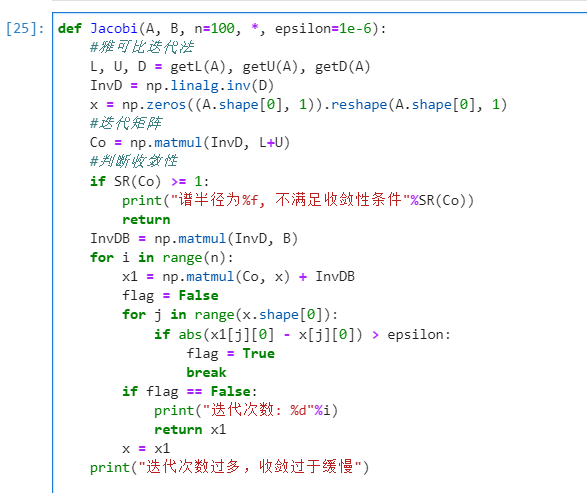
\includegraphics[width=6cm,height=4.8cm]{Jacobi.png}
\caption{Jacobi迭代法代码}
\end{figure}
\newpage
\subsection{收敛性判定及收敛速率的比较}
	实验中,使用迭代矩阵的谱半径$\rho(G)$判断迭代过程的收敛性。书P171.5.(1)和P171.6使用的方程组相同,仅交换了其中两行,却有不相同的谱半径,迭代过程收敛性也不同。这说明可以通过交换方程组的某些行改变迭代过程的收敛性。

\begin{figure}
	\centering
	\subfigure[P171.5.(1)测试结果]{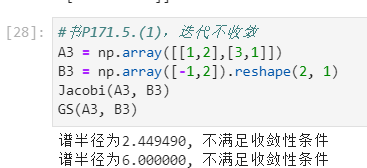
\includegraphics[width=6cm,height=3cm]{5.png}}
	\subfigure[P171.6测试结果]{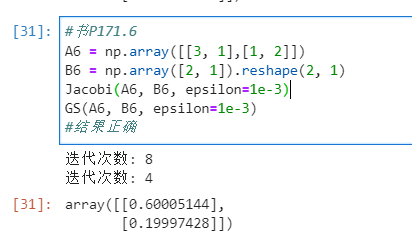
\includegraphics[width=6cm, height=3cm]{6.png}}
	\caption{收敛性的改变}
\end{figure}

	而通过书P170.3和P171.4可以看出,通常雅可比迭代的收敛速率要慢于高斯-塞德尔方法。
\begin{figure}
	\centering
	\subfigure[P170.3测试结果]{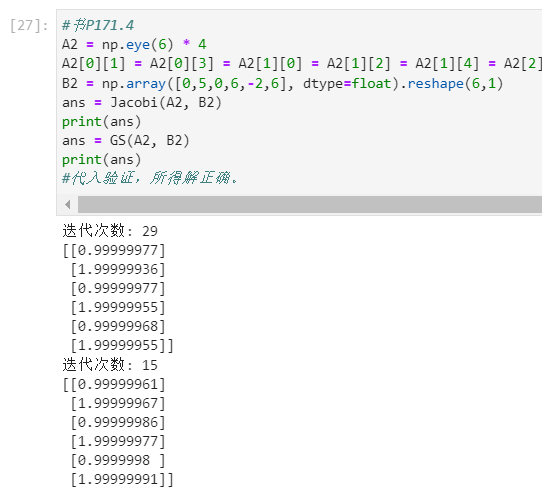
\includegraphics[width=6cm, height=4cm]{实验结果1.png}}
	\subfigure[P171.4测试结果]{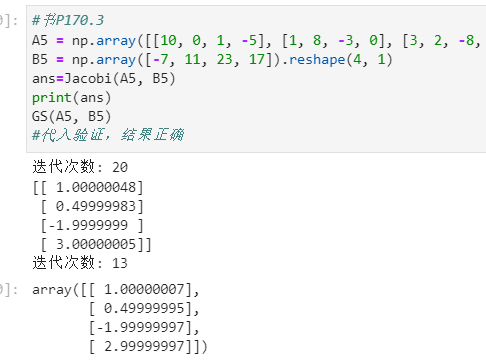
\includegraphics[width=6cm, height=4cm]{实验结果2.png}}
	\caption{收敛速率的不同}
\end{figure}

\section{实验体会}
	这次实验,我对高斯-塞德尔迭代法和雅可比迭代法有了更深入的了解,知道如何判断雅可比迭代和高斯-塞德尔迭代的收敛性,并用两种迭代方法求线性方程组的近似解。此外,这次试验还加强了我的代码能力,并加深了对numpy中矩阵操作的了解。

\end{document}